\begin{figure}[h]
    \centering
    \begin{subfigure}[b]{0.45\textwidth}
        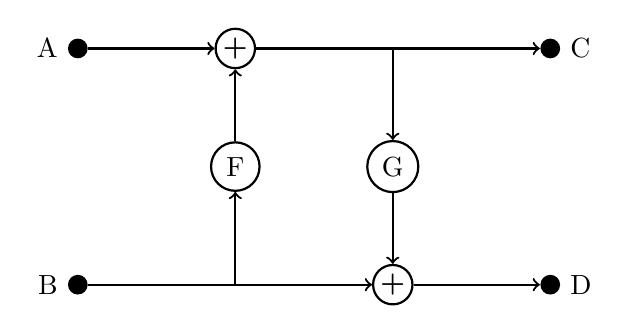
\begin{tikzpicture}[
                dot/.style = {circle, fill, inner sep = 0mm, minimum size = 2.5mm},
                op/.style = {draw, thick, circle, inner sep = 0mm, minimum size = 5mm},
                func/.style = {draw, thick, circle, inner sep = 1mm},
                arr/.style = {draw, thick, ->},
            ]
            \node (A) at (0, 3) [dot, label = left:A] {};
            \node (B) at (0, 0) [dot, label = left:B] {};
            \node (C) at (6, 3) [dot, label = right:C] {};
            \node (D) at (6, 0) [dot, label = right:D] {};

            \node (P1) at (2, 3) [op] {\textbf{+}};
            \node (P2) at (4, 0) [op] {\textbf{+}};

            \node (F) at (2, 1.5) [func] {F};
            \node (G) at (4, 1.5) [func] {G};

            \path[arr] (A) -- (P1);
            \path[arr] (P1) -- (C);
            \path[arr] (B) -- (P2);
            \path[arr] (P2) -- (D);
            \path[arr] (2, 0) -- (F);
            \path[arr] (F) -- (P1);
            \path[arr] (4, 3) -- (G);
            \path[arr] (G) -- (P2);
        \end{tikzpicture}
        \caption{Lifting steps.}
    \end{subfigure}
    \begin{subfigure}[b]{0.5\textwidth}
        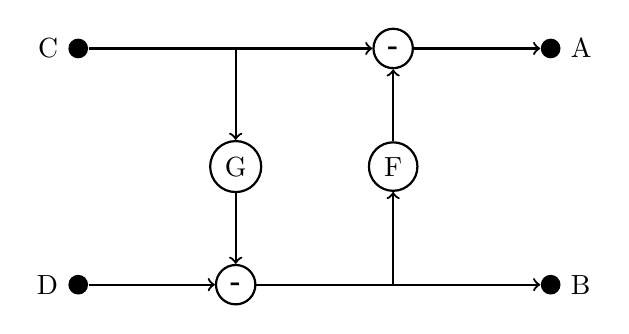
\begin{tikzpicture}[
                dot/.style = {circle, fill, inner sep = 0mm, minimum size = 2.5mm},
                op/.style = {draw, thick, circle, inner sep = 0mm, minimum size = 5mm},
                func/.style = {draw, thick, circle, inner sep = 1mm},
                arr/.style = {draw, thick, ->},
            ]
            \node (A) at (14, 3) [dot, label = right:A] {};
            \node (B) at (14, 0) [dot, label = right:B] {};
            \node (C) at (8, 3) [dot, label = left:C] {};
            \node (D) at (8, 0) [dot, label = left:D] {};

            \node (P1) at (12, 3) [op] {\textbf{-}};
            \node (P2) at (10, 0) [op] {\textbf{-}};

            \node (F) at (12, 1.5) [func] {F};
            \node (G) at (10, 1.5) [func] {G};

            \path[arr] (P1) -- (A);
            \path[arr] (C) -- (P1);
            \path[arr] (P2) -- (B);
            \path[arr] (D) -- (P2);

            \path[arr] (12, 0) -- (F);
            \path[arr] (10, 3) -- (G);
            \path[arr] (F) -- (P1);
            \path[arr] (G) -- (P2);
        \end{tikzpicture}
        \caption{Inverse path.}
    \end{subfigure}
    \caption{Dataflow path of a lifting step and its derived inverse.\label{fig:lift}}
\end{figure}
